\documentclass{beamer}\usepackage[]{graphicx}\usepackage[]{color}
%% maxwidth is the original width if it is less than linewidth
%% otherwise use linewidth (to make sure the graphics do not exceed the margin)
\makeatletter
\def\maxwidth{ %
  \ifdim\Gin@nat@width>\linewidth
    \linewidth
  \else
    \Gin@nat@width
  \fi
}
\makeatother

\definecolor{fgcolor}{rgb}{0.345, 0.345, 0.345}
\newcommand{\hlnum}[1]{\textcolor[rgb]{0.686,0.059,0.569}{#1}}%
\newcommand{\hlstr}[1]{\textcolor[rgb]{0.192,0.494,0.8}{#1}}%
\newcommand{\hlcom}[1]{\textcolor[rgb]{0.678,0.584,0.686}{\textit{#1}}}%
\newcommand{\hlopt}[1]{\textcolor[rgb]{0,0,0}{#1}}%
\newcommand{\hlstd}[1]{\textcolor[rgb]{0.345,0.345,0.345}{#1}}%
\newcommand{\hlkwa}[1]{\textcolor[rgb]{0.161,0.373,0.58}{\textbf{#1}}}%
\newcommand{\hlkwb}[1]{\textcolor[rgb]{0.69,0.353,0.396}{#1}}%
\newcommand{\hlkwc}[1]{\textcolor[rgb]{0.333,0.667,0.333}{#1}}%
\newcommand{\hlkwd}[1]{\textcolor[rgb]{0.737,0.353,0.396}{\textbf{#1}}}%
\let\hlipl\hlkwb

\usepackage{framed}
\makeatletter
\newenvironment{kframe}{%
 \def\at@end@of@kframe{}%
 \ifinner\ifhmode%
  \def\at@end@of@kframe{\end{minipage}}%
  \begin{minipage}{\columnwidth}%
 \fi\fi%
 \def\FrameCommand##1{\hskip\@totalleftmargin \hskip-\fboxsep
 \colorbox{shadecolor}{##1}\hskip-\fboxsep
     % There is no \\@totalrightmargin, so:
     \hskip-\linewidth \hskip-\@totalleftmargin \hskip\columnwidth}%
 \MakeFramed {\advance\hsize-\width
   \@totalleftmargin\z@ \linewidth\hsize
   \@setminipage}}%
 {\par\unskip\endMakeFramed%
 \at@end@of@kframe}
\makeatother

\definecolor{shadecolor}{rgb}{.97, .97, .97}
\definecolor{messagecolor}{rgb}{0, 0, 0}
\definecolor{warningcolor}{rgb}{1, 0, 1}
\definecolor{errorcolor}{rgb}{1, 0, 0}
\newenvironment{knitrout}{}{} % an empty environment to be redefined in TeX

\usepackage{alltt}
\usetheme{berkeley}
\usecolortheme{albatross}
\IfFileExists{upquote.sty}{\usepackage{upquote}}{}
\begin{document}

\title{Cumulative Sentiment Line Chart}
\author{Andrew Mayo}

\begin{frame}
  \titlepage
\end{frame}

\begin{frame}
  \frametitle{Outline}
    \tableofcontents
\end{frame}


\section{Install and Load Libraries}
\begin{frame}[fragile]
  \frametitle{Install and Load Libraries}
    \begin{itemize}
      \item<1->
\begin{knitrout}
\definecolor{shadecolor}{rgb}{0.969, 0.969, 0.969}\color{fgcolor}\begin{kframe}
\begin{alltt}
\hlkwd{library}\hlstd{(dplyr)}
\end{alltt}
\end{kframe}
\end{knitrout}
      \item<2->
\begin{knitrout}
\definecolor{shadecolor}{rgb}{0.969, 0.969, 0.969}\color{fgcolor}\begin{kframe}
\begin{alltt}
\hlkwd{library}\hlstd{(tidytext)}
\end{alltt}
\end{kframe}
\end{knitrout}
      \item<3->
\begin{knitrout}
\definecolor{shadecolor}{rgb}{0.969, 0.969, 0.969}\color{fgcolor}\begin{kframe}
\begin{alltt}
\hlkwd{library}\hlstd{(gutenbergr)}
\end{alltt}
\end{kframe}
\end{knitrout}
      \item<4->
\begin{knitrout}
\definecolor{shadecolor}{rgb}{0.969, 0.969, 0.969}\color{fgcolor}\begin{kframe}
\begin{alltt}
\hlkwd{library}\hlstd{(ggplot2)}
\end{alltt}
\end{kframe}
\end{knitrout}
      \item<5->
\begin{knitrout}
\definecolor{shadecolor}{rgb}{0.969, 0.969, 0.969}\color{fgcolor}\begin{kframe}
\begin{alltt}
\hlkwd{library}\hlstd{(stringr)}
\end{alltt}
\end{kframe}
\end{knitrout}
    \end{itemize}
\end{frame}

\section{Access Project Gutenberg}
\begin{frame}[fragile]
  \frametitle{Access Project Gutenberg}
\begin{knitrout}
\definecolor{shadecolor}{rgb}{0.969, 0.969, 0.969}\color{fgcolor}\begin{kframe}
\begin{alltt}
\hlkwd{gutenberg_works}\hlstd{(}\hlkwd{str_detect}\hlstd{(title,} \hlstr{"Frankenstein"}\hlstd{))}
\end{alltt}
\begin{verbatim}
## # A tibble: 1 x 8
##   gutenberg_id                                   title
##          <int>                                   <chr>
## 1           84 Frankenstein; Or, The Modern Prometheus
## # ... with 6 more variables: author <chr>, gutenberg_author_id <int>,
## #   language <chr>, gutenberg_bookshelf <chr>, rights <chr>,
## #   has_text <lgl>
\end{verbatim}
\end{kframe}
\end{knitrout}
\end{frame}

\section{Download Dracula and Sentiments}
\begin{frame}[fragile]
  \frametitle{Download Dracula and Sentiments}
\begin{knitrout}
\definecolor{shadecolor}{rgb}{0.969, 0.969, 0.969}\color{fgcolor}\begin{kframe}
\begin{alltt}
\hlstd{afinn} \hlkwb{<-} \hlkwd{get_sentiments}\hlstd{(}\hlstr{"afinn"}\hlstd{)}
\hlstd{frank} \hlkwb{<-} \hlkwd{gutenberg_download}\hlstd{(}\hlnum{84}\hlstd{)}
\end{alltt}
\end{kframe}
\end{knitrout}
\end{frame}


\section{Unpacking Words}
\begin{frame}[fragile]
  \frametitle{Unpacking Words}
\begin{knitrout}
\definecolor{shadecolor}{rgb}{0.969, 0.969, 0.969}\color{fgcolor}\begin{kframe}
\begin{alltt}
\hlstd{f_words} \hlkwb{<-} \hlstd{frank}\hlopt
    \hlkwd{unnest_tokens}\hlstd{(word,text)}
\hlkwd{colnames}\hlstd{(f_words)}
\end{alltt}
\begin{verbatim}
## [1] "gutenberg_id" "word"
\end{verbatim}
\begin{alltt}
\hlstd{f_words}\hlopt{$}\hlstd{word[}\hlnum{500}\hlstd{]}
\end{alltt}
\begin{verbatim}
## [1] "may"
\end{verbatim}
\end{kframe}
\end{knitrout}
\end{frame}

\section{Word Numbers}
\begin{frame}[fragile]
  \frametitle{Adding Word Numbers}
\begin{knitrout}
\definecolor{shadecolor}{rgb}{0.969, 0.969, 0.969}\color{fgcolor}\begin{kframe}
\begin{alltt}
\hlkwd{nrow}\hlstd{(f_words)}
\end{alltt}
\begin{verbatim}
## [1] 75175
\end{verbatim}
\begin{alltt}
\hlstd{f_words}\hlopt{$}\hlstd{word_number} \hlkwb{<-} \hlnum{1}\hlopt{:}\hlnum{75175}
\end{alltt}
\end{kframe}
\end{knitrout}
\end{frame}

\section{The Inner-join}
\begin{frame}[fragile]
  \frametitle{The Inner-join}
\begin{knitrout}
\definecolor{shadecolor}{rgb}{0.969, 0.969, 0.969}\color{fgcolor}\begin{kframe}
\begin{alltt}
\hlstd{frank_sent} \hlkwb{<-} \hlkwd{inner_join}\hlstd{(afinn, f_words)}
\end{alltt}


{\ttfamily\noindent\itshape\color{messagecolor}{\#\# Joining, by = "{}word"{}}}\begin{alltt}
\hlstd{frank_sent}\hlopt{$}\hlstd{gutenberg_id} \hlkwb{<-} \hlkwa{NULL}
\hlkwd{head}\hlstd{(frank_sent)}
\end{alltt}
\begin{verbatim}
## # A tibble: 6 x 3
##        word score word_number
##       <chr> <int>       <int>
## 1   abandon    -2       30647
## 2   abandon    -2       69663
## 3 abandoned    -2        1996
## 4 abandoned    -2       41559
## 5 abandoned    -2       74516
## 6     abhor    -3       30461
\end{verbatim}
\end{kframe}
\end{knitrout}
\end{frame}

\section{Arranging Words}
\begin{frame}[fragile]
  \frametitle{Arranging Words in Book Order}
\begin{knitrout}
\definecolor{shadecolor}{rgb}{0.969, 0.969, 0.969}\color{fgcolor}\begin{kframe}
\begin{alltt}
\hlstd{frank_sent} \hlkwb{<-} \hlstd{frank_sent}\hlopt
          \hlkwd{arrange}\hlstd{(word_number)}
\hlkwd{head}\hlstd{(frank_sent)}
\end{alltt}
\begin{verbatim}
## # A tibble: 6 x 3
##         word score word_number
##        <chr> <int>       <int>
## 1    rejoice     4          24
## 2         no    -1          28
## 3   disaster    -2          29
## 4       evil    -3          43
## 5       dear     2          57
## 6 confidence     2          64
\end{verbatim}
\end{kframe}
\end{knitrout}

\end{frame}

\section{Cumulative Sentiment}
\begin{frame}[fragile,allowframebreaks]
  \frametitle{Getting the Cumulative Sentiment}
\begin{knitrout}
\definecolor{shadecolor}{rgb}{0.969, 0.969, 0.969}\color{fgcolor}\begin{kframe}
\begin{alltt}
\hlstd{frank_sent}\hlopt{$}\hlstd{accum_sent} \hlkwb{<-} \hlkwd{cumsum}\hlstd{(frank_sent}\hlopt{$}\hlstd{score)}
\hlkwd{head}\hlstd{(frank_sent)}
\end{alltt}
\begin{verbatim}
## # A tibble: 6 x 4
##         word score word_number accum_sent
##        <chr> <int>       <int>      <int>
## 1    rejoice     4          24          4
## 2         no    -1          28          3
## 3   disaster    -2          29          1
## 4       evil    -3          43         -2
## 5       dear     2          57          0
## 6 confidence     2          64          2
\end{verbatim}
\end{kframe}
\end{knitrout}


\end{frame}

\section{Line Plot}
\begin{frame}[fragile,allowframebreaks]
  \frametitle{Changing Sentiment Throughout Frankenstein}
\begin{knitrout}
\definecolor{shadecolor}{rgb}{0.969, 0.969, 0.969}\color{fgcolor}\begin{kframe}
\begin{alltt}
 \hlstd{plot} \hlkwb{<-} \hlkwd{ggplot}\hlstd{()}\hlopt{+}
\hlkwd{geom_line}\hlstd{(}\hlkwc{data} \hlstd{= frank_sent,}
          \hlkwd{aes}\hlstd{(}\hlkwc{x} \hlstd{= word_number,}
              \hlkwc{y} \hlstd{= accum_sent))}
\end{alltt}
\end{kframe}
\end{knitrout}

\framebreak
\begin{knitrout}
\definecolor{shadecolor}{rgb}{0.969, 0.969, 0.969}\color{fgcolor}
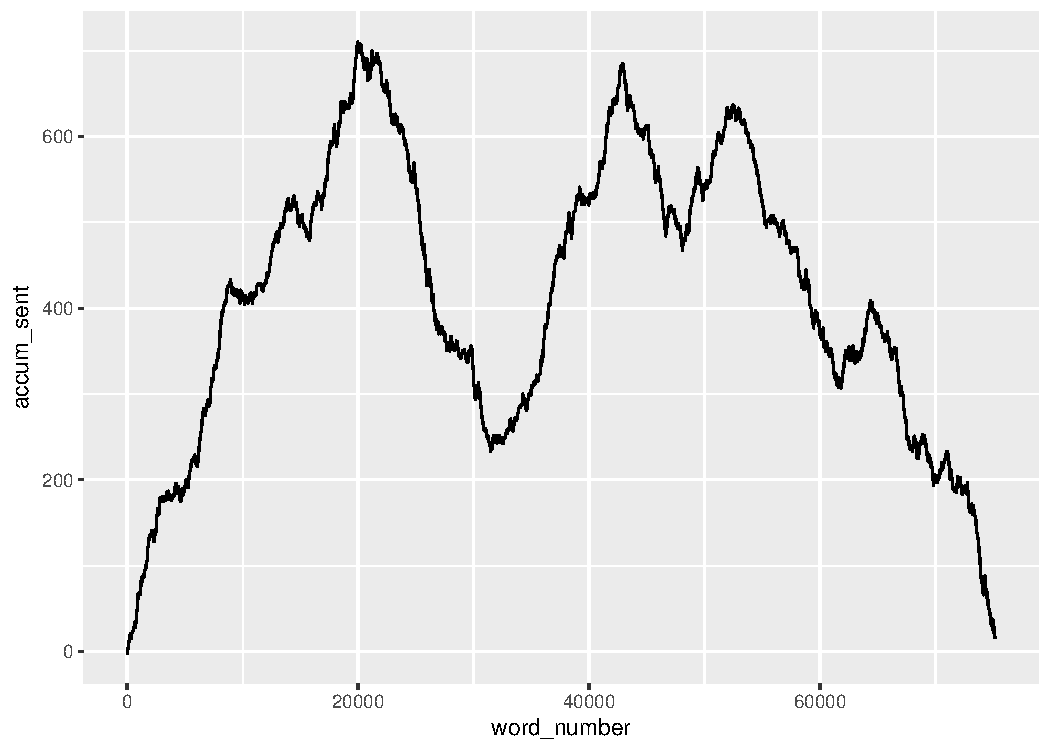
\includegraphics[width=\maxwidth]{figure/unnamed-chunk-14-1} 

\end{knitrout}

\end{frame}
\end{document}
